\documentclass[10pt,pdf,hyperref={unicode}]{beamer}

\usepackage{graphicx}
\graphicspath{{./figs/}}

\mode<presentation> {
	\usetheme{Warsaw}
	  % or ...
	  
	\setbeamercovered{transparent}
  % or whatever (possibly just delete it)
}

\usepackage[english]{babel}
\usepackage[utf8x]{inputenc}

%\usepackage{amsmath}
\usepackage{bm}
\usepackage{tikz}
\usepackage{pgfplots}

\title[] % (optional, use only with long paper titles)
{Modelling dynamic processes in a nuclear reactor
by state change modal method}

%\subtitle
%{Include Only If Paper Has a Subtitle}

\author[] % (optional, use only with lots of authors)
{{Aleksandr Vasilev}}
% - Give the names in the same order as the appear in the paper.
% - Use the \inst{?} command only if the authors have different
%   affiliation.

\institute[Universities of Somewhere and Elsewhere] % (optional, but mostly needed)
{
North-Eastern Federal University in Yakutsk \\
Multiscale Model Reduction and High Perfomance Computing Laboratory
}

% - Use the \inst command only if there are several affiliations.
% - Keep it simple, no one is interested in your street address.

\date[July 22, 2017] % (optional, should be abbreviation of conference name)
{July 22, 2017, Yakutsk}
% - Either use conference name or its abbreviation.
% - Not really informative to the audience, more for people (including
%   yourself) who are reading the slides online

\subject{Theoretical Computer Science}
% This is only inserted into the PDF information catalog. Can be left
% out. 

% ����� � ���������
\graphicspath{{./figs/}}
\newcommand{\grad}{\mathop{\rm grad}\nolimits}
\renewcommand{\div}{\mathop{\rm div}\nolimits}
\newcommand{\const}{\mathop{\rm const}\nolimits}

\begin{document}

\begin{frame}
  \titlepage
\end{frame}

%{
%  \begin{frame}<beamer>
%    \tableofcontents
%  \end{frame}
%}

%\section{Introduction}
%\begin{frame}{Introduction}
%\begin{footnotesize}
%\begin{itemize}
%\item
%Quasistatic method. 
%In this case, an approximate solution is represented as a product of two functions: one of which depends on the time and is related to the amplitude, the second (shape function) describes the spatial distribution. The shape function is often associated with the fundamental eigenfunction of certain eigenvalue problems for neutron diffusion equations. 
%\item
%When using the quasistatic method, the problem is significantly simplified, thus, it is doubtful to obtain good accuracy for an approximate solution, in particular, in dynamic regimes with a complex redistribution of the neutron flux. For this reason, the more general approach of the modal method has been successfully developed.
%In this case, the solution is represented in the form of a sum of several dominant eigenvalues with time-dependent coefficients.
%\item
%Nonstationary processes can naturally be described on the basis of the approximate solution expansion in time-eigenvalue of  $\alpha$-eigenvalue problem.
%We deal with an unbound system of equations for the coefficients. It should also be noted that the eigenvalues are complex for both   $\lambda$- and 
%$\alpha$-eigenvalue problem. To set the initial state, this leads to the need to solve the appropriate adjoint spectral problems.
%\item
%We formulate a general strategy for the approximate solution of nonstationary problems of neutron transport in nuclear reactors, which is oriented to fast real-time calculations using the State Change Modal (SCM) method. 
%
%\end{itemize}
%\end{footnotesize}
%\end{frame}

\section{Problem description}
\subsection{Multigroup diffusion approximation}
\begin{frame}{Multigroup diffusion approximation}
Instantaneous neutrons:
\begin{eqnarray*}
\frac{1}{v_g} \frac{\partial \phi_g}{\partial t} - \nabla \cdot D_g \nabla \phi_g + \Sigma_{rg} \phi_g - \sum_{g\neq g'=1}^{G} \Sigma_{s,g'\rightarrow g} \phi_{g'} = 
\\ 
= (1-\beta) \chi_g \sum_{g'=1}^{G} \nu \Sigma_{fg'} \phi_{g'} + \widetilde{\chi}_g \sum_{m=1}^{M} \lambda_m c_m , \quad 
 g = 1,2, ..., G .
\end{eqnarray*}
Delayed neutrons:
\begin{eqnarray*}
 \frac{\partial c_m}{\partial t} + \lambda_m c_m = \beta_m \sum_{g=1}^{G} \nu \Sigma_{fg} \phi_g,
 \quad m = 1,2, ..., M, 
\end{eqnarray*}
where $\beta_m$ is is a fraction of delayed neutrons of $m$ type, and
\[
 \beta = \sum_{m=1}^{M} \beta_m .
\] 

\end{frame}

\subsection{Initial and boundary conditions}
\begin{frame}{Initial and boundary conditions}

The albedo-type conditions are set at the boundary $\partial \Omega$ of the area $\Omega$:
\begin{eqnarray*}
 D_g\frac{\partial \phi_g}{\partial n} + \gamma_g \phi_g = 0, \quad 
 \quad g = 1,2, ..., G.
\end{eqnarray*}

We consider boundary problem with albedo boundary condition and the initial condition:
\begin{eqnarray*}
 \phi_g(\bm x,0) = \phi_g^0(\bm x), 
  \quad  g = 1,2, ..., G ,
 \quad   c_m(\bm x,0) = c_m^0(\bm x), 
  \quad  m = 1,2, ..., M .
\end{eqnarray*}

\end{frame}

\subsection{Operator formulation}
\begin{frame}{Operator formulation}
\begin{small}
Define vectors $\bm \phi = \{\phi_1, \phi_2, ..., \phi_G\}$, $\bm c = \{c_1, c_2, ..., c_M\}$ and matrix: 
\[
\begin{split}
& V = (v_{g g'}), \quad v_{g g'} = \delta_{g g'} v_g^{-1}, 
\quad\phantom{1234567}
 D = (d_{g g'}), \quad d_{g g'} = - \delta_{g g'} \nabla \cdot D_g \nabla, \\
& S = (s_{g g'}), \quad  s_{g g'} = \delta_{g g'} \Sigma_g - \Sigma_{s,g'\rightarrow g}, \quad
 R = (r_{g g'}), \quad  r_{g g'} = (1-\beta)\chi_g \nu \Sigma_{fg'}, \\
& B = (b_{g m}), \quad b_{g m} = \widetilde{\chi}_g \lambda_m, \quad\phantom{1234567890}
 \Lambda = (\lambda_{m m'}), \quad  \lambda_{m m'} = \lambda_m \delta_{m m'}, \\
& Q = (q_{mg}), \quad  q_{mg} = \beta_m \nu \Sigma_{fg},
 \quad \phantom{1234567}
 g, g' = 1,2, ..., G, \quad m, m' = 1,2, ....,M.  
\end{split}
\]
Using the set definitions, we get boundary problem in operator formulation:
\begin{eqnarray*}
V \frac{d \bm \phi}{d t} + (D+S) \bm \phi = R \bm \phi + B\bm c,
\\
\frac{d \bm c}{d t} + \Lambda \bm c = Q \bm \phi. 
\end{eqnarray*}  
The Cauchy problem is solved under initial conditions:
\begin{eqnarray*}
\bm \phi(0) = \bm \phi^0, \quad  \bm c(0) = \bm c^0,
\end{eqnarray*}  
where $L = (l_{g g'}), \quad l_{g g'} = \delta_{g g'} \gamma_g, \quad \bm \phi^0 = \{ \phi_1^0,  \phi_2^0, ...,  \phi_G^0 \}, \quad
\bm c^0 = \{ c_1^0,  c_2^0, ...,  c_M^0 \}$.
\end{small}
\end{frame}

%\subsection{Discretization}
%\begin{frame}{Finite element method}
%\begin{footnotesize}
%Let $H^1(\Omega)$ -- sobolev space, $v \in H^1$: $v^2$ and $\vert\nabla v\vert^2$ have a finite integral in $\Omega$. For $\bm v = \{v_1, v_2, ..., v_d\}$ define $V^d = [H^1(\Omega)]^d$. For test functions use notations $\bm \xi  = \{\xi_1, \xi_2, ..., \xi_G\}$, $\bm \zeta  = \{\zeta_1, \zeta_2, ..., \zeta_M\}$.\\
%In variation formulation we are looking for $\bm \phi \in V^D, \ \bm c \in V^M$ such that:
%\begin{eqnarray*}
%\begin{split}
%\int_\Omega \left (V \frac{\bm\phi^{n+1}-\bm\phi^n}{\tau} + S
%\bm \phi^{n+1} \right )\bm \xi  d\bm x 
%+ \int_{\Omega} \sum_{g=1}^{G} D_G \nabla \phi^{n+1}_g \nabla  \xi_g d\bm x + \\
%+ \int_{\partial \Omega} \sum_{g=1}^{G} \gamma_g \phi^{n+1}_g \xi_g d\bm x
%= \int_\Omega R \bm \phi^{n+1}\bm \xi d\bm x + \int_\Omega B\bm c^{n+1}\bm \xi d\bm x,
%\\
%\int_\Omega \bm{c}^{n+1}\bm \zeta d\bm x = \int_\Omega \widetilde{\Lambda}\bm{c}^{n}\bm \zeta  d\bm x + \int_\Omega \tau Q \bm{\phi}^{n+1}\bm \zeta  d\bm x
%\end{split}
%\end{eqnarray*}
%for all $\bm \xi  \in V^D, \ \bm \zeta  \in V^M$.
%\\
%Let introduce a discrete function spaces $V_h^D \subset V^D$, $V_h^M \subset V^M$ and define discrete variational problem.
%
%The standard Lagrangian finite elements of degree p =
%1, 2 and 3 are used.
%\end{footnotesize}
%\end{frame}

\section{State change modal method}
\subsection{State change scheme}
\begin{frame}{State change scheme}
The state of the reactor is characterized by the constant coefficients of the system of multigroup diffusion equations.
\begin{figure}[ht]
\begin{center}
\vspace{5mm} 
    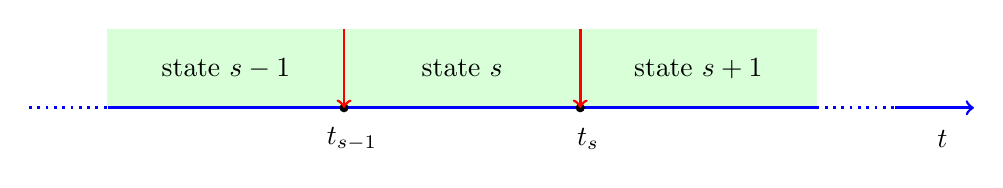
\begin{tikzpicture}
      \filldraw [color=green!15] (0,0) rectangle +(9,1);
      \draw [dotted, line width=1, color=blue] (-1,0) -- (0,0);
      \draw [line width=1, color=blue] (0,0) -- (9,0);
      \draw [dotted, line width=1, color=blue] (9,0) -- (10,0);
      \draw [->, line width=1, color=blue] (10,0) -- (11,0);
      \filldraw [black] (3,0) circle (0.05);
      \filldraw [black] (6,0) circle (0.05);
      \draw  (1.5,0.5) node {state $s-1$};  
      \draw  (4.5,0.5) node {state $s$};  
      \draw  (7.5,0.5) node {state $s+1$};  
      \draw  (3.1,-0.4) node {$t_{s-1}$}; 
      \draw  (6.1,-0.4) node {$t_{s}$}; 
      \draw  (10.6,-0.4) node {$t$}; 
      \draw [->, line width=1, color=red] (3,1) -- (3,0);
      \draw [->, line width=1, color=red] (6,1) -- (6,0);
    \end{tikzpicture}
  \end{center}
\end{figure}
Dynamic processes in a nuclear reactor can be considered as a change of states. 
At a certain time $t = t_s, \ s = 1,2, ...$ an instantaneous change of state occurs. 
The state $s$ is defined by the parameters in equations:
\[
 V(t) = V(t_s), \quad  D(t) = D(t_s), \quad  S(t) = S(t_s), \quad  R(t) = R(t_s), \quad  B(t) = B(t_s),
\] 
\[
 \Lambda(t) = \Lambda(t_s), \quad  Q(t) = Q(t_s),
 \quad t_{s-1} < t \leq t_s, \quad s = 1,2, ... 
\] 
\end{frame}

%\subsection{Modal approximation}
%\begin{frame}{Modal approximation}
%An approximate description of the non-stationary process at a separate stage is based on modal approximation. An approximate solution is sought in the form of decomposition in eigenfunctions of time and $\alpha$-eigenvalue problem.
%
%Let's $\bm u = \{\bm \phi, \bm c\}, \quad \bm \phi(t_{s-1}) = \bm \phi^s,
% \quad   \bm c(t_{s-1}) = \bm c^s$ .
%In a separate stage s the following system is considered
%\begin{eqnarray*}
% \bm B \frac{d \bm u}{d t} + \bm A \bm u = 0,
% \quad t_{s-1} < t \leq t_s,
%\end{eqnarray*}
%with constants
%\[
% \bm A = 
% \begin{pmatrix}
% D(t_s)+S(t_s) - R(t_s) &  - B(t_s) \\
% - Q(t_s) & \Lambda(t_s) 
% \end{pmatrix} ,
% \quad  \bm B = 
% \begin{pmatrix}
% V(t_s) & 0 \\
% 0 & I 
% \end{pmatrix}.
%\] 
%Supplemented by the corresponding initial condition
%\begin{eqnarray*}
% \bm u(t_{s-1}) = \bm u^s .
%\end{eqnarray*}
%The main feature of the problems we are considering is that the matrices $\bm A_h$ and $\bm B_h$ 
%are real and asymmetric.
%\end{frame}

%\begin{frame}{Modal approximation}
%\begin{footnotesize}
%The modal approximation corresponds to the representation of the approximate solution  ($\bm u_h \approx \bm u_N$) of problem  in the following form
%\[
% \bm u_N(\bm x, t) =
% \sum_{n=1}^{N} a_n(t) \bm w_n(\bm x),
%\]
%where $N$ is the number of dominant eigenvalues of the spectral problem, 
%$\bm w_n(\bm x)$ --- corresponding eigenfunctions.
%
%Let us define eigenfunctions and eigenvalues as the solution of the  $\alpha$-eigenvalue problem:
%\[
% \bm A_h \bm v = \lambda  \bm B_h \bm v .
%\]
%In the simplest case all eigenvalues of the spectral problem are real:
%\[
% \lambda_1 \leq \lambda_2 \leq ... \leq \lambda_{N_h} .
%\] 
%Under these conditions the general solution of equation is
%\[
% \bm u_h(\bm x, t) =
% \sum_{n=1}^{N_h} b_n \exp(-\lambda_n (t-t_{s-1})) \bm v_n(\bm x) , 
%\]
%that is 
%\[
% a_n(t) = b_n \exp(-\lambda_n (t-t_{s-1})) ,
% \quad \bm w_n(\bm x) = \bm v_n(\bm x),
% \quad n = 1,2, ..., N .  
%\] 
%\end{footnotesize}
%\end{frame}

%\begin{frame}
%In the general case, eigenfunctions and eigenvalues of the spectral problem are complex.
%Taking into account the validity of the matrix coefficients  $\bm A_h, \ \bm B_h$ complex eigenvalues appear as pairs of complex conjugate numbers. For example, we have a pair of $n,n+1$: 
%\[
% \lambda_{n+1} = \mathrm{Re} \lambda_n - i \mathrm{Im} \lambda_n . 
%\] 
%Then we obtain
%\[
%\begin{split}
% a_n(t) \bm w_n(\bm x) & = b_n \mathrm{Re} \big ( \exp(-\lambda_n (t-t_{s-1})) \bm v_n(\bm x) \big ), \\
% a_{n+1}(t) \bm w_{n+1}(\bm x) & = b_{n+1} \mathrm{Im} \big ( \exp(-\lambda_n (t-t_{s-1})) \bm v_n(\bm x) \big ) .
%\end{split}
%\] 
%A special attention should be paid to define the coefficients $a_n(t_{s-1}) = b_n, \ n = 1,2, ..., N$.
%For this, the initial condition is involved. For example, in the case of real eigenvalues, we have
%\[
% \bm u_h^s (\bm x) = \sum_{n=1}^{N_h} b_n \bm v_n(\bm x) .
%\] 
%This representation is not very suitable for practical use with modal approximation, when we work only with dominant eigenfunctions.  
%\end{frame}

\subsection{Time scale processes}
\begin{frame}{Time scale processes}
The initial condition includes two components  $\bm u_h^s (\bm x) = (\bm \phi_h^s (\bm x), \bm c_h^s (\bm x))$.
Dynamic behaviour of these components is due to different time-scale processes. Delayed neutrons source determines \textbf{slow processes}, when  $\bm c(\bm x,t)$ changes slightly with the reactor state change. In contrast, neutron flux $\bm \phi(\bm x,t)$ determines \textbf{fast processes} when the reactor state changes. By virtue of this separation of dynamic processes, we model the slow phase of the dynamics of the reactor with modal approximation and orientate ourselves on the approximate prediction of the initial state for delayed neutrons, only the function  $\bm c_h^s (\bm x)$ is approximated. The approximation  $\bm \phi_h^s (\bm x)$ is not of interest to us; we do not model a fast phase of the state change.
\end{frame}

%\subsection{Adjoint spectral problem}
%\begin{frame}{Adjoint spectral problem}
%Consider the adjoint spectral problem 
%\[
% \bm A_h^T \widetilde{\bm v}  = \lambda  \bm B_h^T \widetilde{\bm v} .
%\]
%The eigenfunctions of problems  are orthogonal  in the sense of the equality
%\[
%  (\bm B_h \bm v_n, \widetilde{\bm v}_m)= 0, 
%  \quad m \neq n,
%  \quad m, n = 1,2, ..., N_h.
%\] 
%In view of this, one can obtain
%\[
% b_n = \frac{1}{(\bm B_h \bm v_n, \widetilde{\bm v}_n)} (\bm u_h^s, \bm B_h \widetilde{\bm v}_n),
% \quad n = 1,2, ..., N_h .  
%\]
%In the approximate solution of problem  only the first $N$ coefficients  $b_n$ are used:
%\[
% \bm c_h^s (\bm x) \approx  \sum_{n=1}^{N} b_n \bm c_n(\bm x) ,
%\]
%where $\bm v_n (\bm x) = (\bm \phi_n (\bm x), \bm c_n (\bm x))$.
%In this case, the spectral problems are solved for $N$ dominant eigenvalues.
%\end{frame}

\begin{frame}{Computation scheme}
\begin{description}
\item[Off-line calculation.] 
Calculation of the coefficients of the mathematical model of the multigroup diffusion approximation for the isolated reactor states, which is performed in advance. 
The status passport also includes calculated dominant eigenvalues and eigenfunctions of the  $\alpha$-eigenvalue problem. 
These data can be supplemented by dominant eigenvalues and eigenvalues of the conjugate eigenvalue problem.
\item[On-line calculation.]
Real-time modeling is carried out on the basis of the modal solution of the problem.
The coefficients in the representation are calculated from the initial condition. 
The solution for other time intervals is determined according to modal approximation.   
\end{description}  
\end{frame}

\section{The test}
\subsection{Benchmark}
\begin{frame}{VVER-1000 benchmark}
The dynamics of the VVER-1000 reactor during the transition from the supercritical mode to the subcritical mode
\begin{columns}[]
\column{0.5\textwidth}
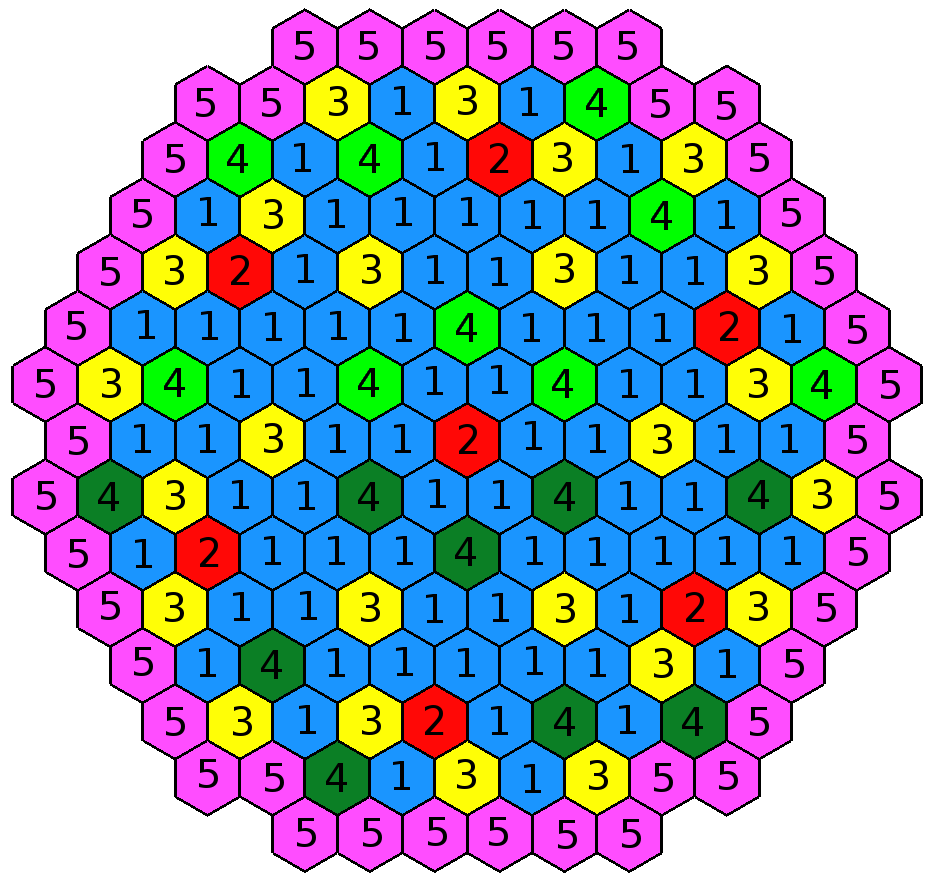
\includegraphics[width=1\linewidth]{geo.png}
\column{0.5\textwidth}
\begin{itemize}
\item two-dimensional and two-group approximation
\item one groups of delayed neutrons
\item the number of triangles per cassette $\kappa$ varies from 6 to 96
\item order of finite elements $p$ varies from 1 to 3
\item two types of perturbation
\end{itemize}
\end{columns}
\end{frame}

%\subsection{Supercritical state}
%\begin{frame}{Supercritical state: $\alpha$-eigenvalue problem}
%\begin{table}[h]
%\caption{Eigenvalues $\alpha_n = \lambda_n^{(\alpha )}, \ n = 1,2, ..., 5$}
%\label{t-2}
%\begin{center}
%\begin{tabular}{cccccc}
%\hline
%$p$ & $\kappa$ & $\alpha_1$ &  $\alpha_2, \alpha_3$ &  $\alpha_4, \alpha_5$ \\ 
%\hline
%& 6 & -0.22557  & 0.04241 $\mp$ 3.08808e-06$i$  & 0.06588 $\mp$ 4.80449e-07$i$  \\
%1 & 24 & -0.82690  & 0.03777 $\mp$ 5.37884e-06$i$  & 0.06489 $\mp$ 1.37315e-06$i$ \\
%& 96 & -1.74998  & 0.03619 $\mp$ 5.69002e-06$i$  & 0.06456 $\mp$ 1.40299e-06$i$ \\
%\hline
%& 6 & -2.10154  & 0.03592 $\mp$ 4.96474e-06$i$  & 0.06452 $\mp$ 1.21320e-06$i$ \\
%2 & 24 & -2.46601  & 0.03562 $\mp$ 5.78277e-06$i$  & 0.06445 $\mp$ 1.40897e-06$i$ \\
%& 96 & -2.50375  & 0.03559 $\mp$ 5.80693e-06$i$  & 0.06444 $\mp$ 1.41324e-06$i$ \\
%\hline
%& 6 & -2.47975  & 0.03561 $\mp$ 5.83718e-06$i$  & 0.06445 $\mp$ 1.41869e-06$i$ \\
%3 & 24 & -2.50294  & 0.03559 $\mp$ 5.80783e-06$i$  & 0.06444 $\mp$ 1.41341e-06$i$ \\
%& 96 & -2.51280  & 0.03558 $\mp$ 5.80954e-06$i$  & 0.06444 $\mp$ 1.41362e-06$i$ \\
%\hline
%\end{tabular}
%\end{center}
%\end{table}
%\end{frame}

%\begin{frame}
%\begin{table}[h]
%\caption{Eigenvalues $\alpha_n = \lambda_n^{(\alpha )}, \ n = 6,7, ..., 10$}
%\label{t-3}
%\begin{center}
%\begin{tabular}{ccccccc}
%\hline
%$p$ & $\kappa$ & $\alpha_6$ &  $\alpha_7$ & $\alpha_8$ &  $\alpha_9, \alpha_{10}$ \\ 
%\hline
%& 6 & 0.07107  & 0.07214  & 0.07323  & 0.07397 $\mp$ 2.04990e-08$i$ \\
%1 & 24 & 0.07050  & 0.07167  & 0.07283  & 0.07362 $\mp$ 3.65907e-08$i$ \\
%& 96 & 0.07033  & 0.07152  & 0.07269  & 0.07351 $\mp$ 3.91936e-08$i$  \\
%\hline
%& 6  & 0.07030  & 0.07151  & 0.07268  & 0.07349 $\mp$ 3.69824e-08$i$ \\
%2 & 24 & 0.07027  & 0.07147  & 0.07265  & 0.07347 $\mp$ 4.03121e-08$i$ \\
%& 96  & 0.07026  & 0.07147  & 0.07265  & 0.07347 $\mp$ 4.02324e-08$i$ \\
%\hline
%& 6 & 0.07027  & 0.07147  & 0.07265  & 0.07347 $\mp$ 4.02573e-08$i$ \\
%3 & 24 & 0.07026  & 0.07147  & 0.07265  & 0.07347 $\mp$ 4.02248e-08$i$ \\
%& 96 & 0.07026  & 0.07147  & 0.07265  & 0.07347 $\mp$ 4.02332e-08$i$ \\
%\hline
%\end{tabular}
%\end{center}
%\end{table}
%\end{frame}

\begin{frame}
\begin{figure}[!h]
	\begin{center}
		\begin{minipage}{0.49\linewidth}
			\center{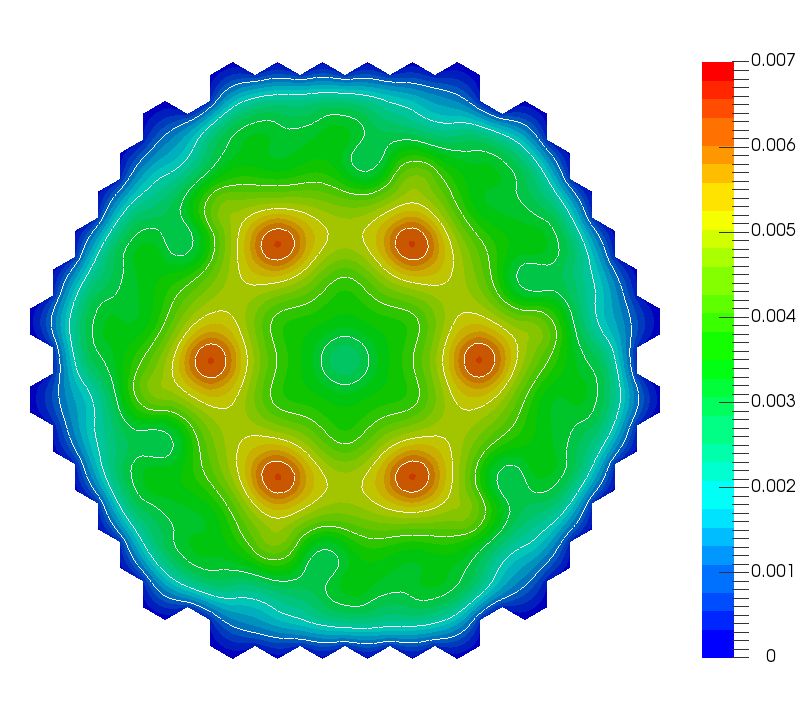
\includegraphics[width=1\linewidth]{4-1.png}} \\
		\end{minipage}
		\hfill
		\begin{minipage}{0.49\linewidth}
			\center{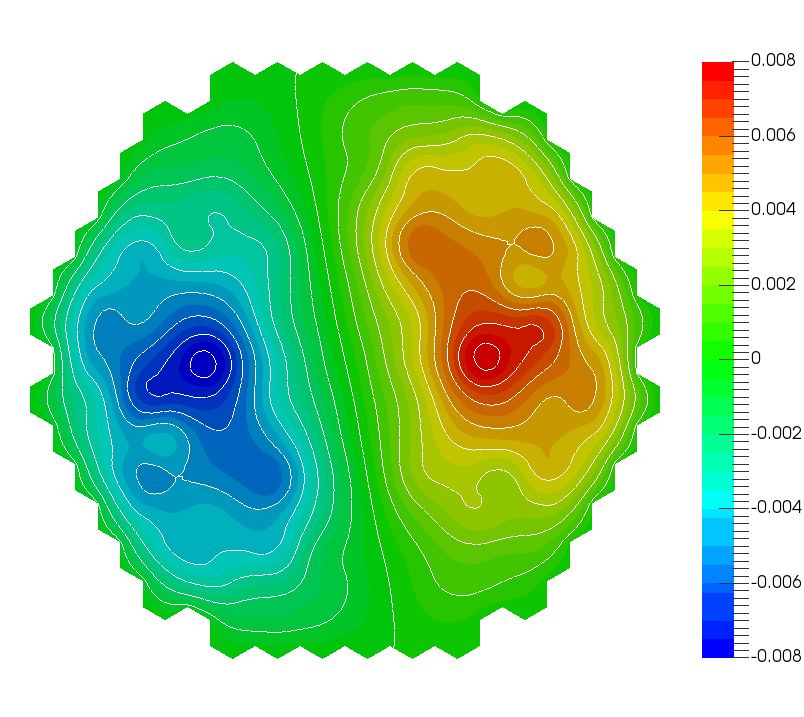
\includegraphics[width=1\linewidth]{4-2.png}} \\
		\end{minipage}
	\caption{The eigenfunction $\varphi^{(1)}_1$ (left) and real part of eigenfunctions $\varphi^{(2)}_1, \ \varphi^{(3)}_1$  (right).}
		\label{fig:4}
	\end{center}
\end{figure}
\end{frame}

%\begin{frame}
%\begin{figure}[!h]
%	\begin{center}
%		\begin{minipage}{0.49\linewidth}
%			\center{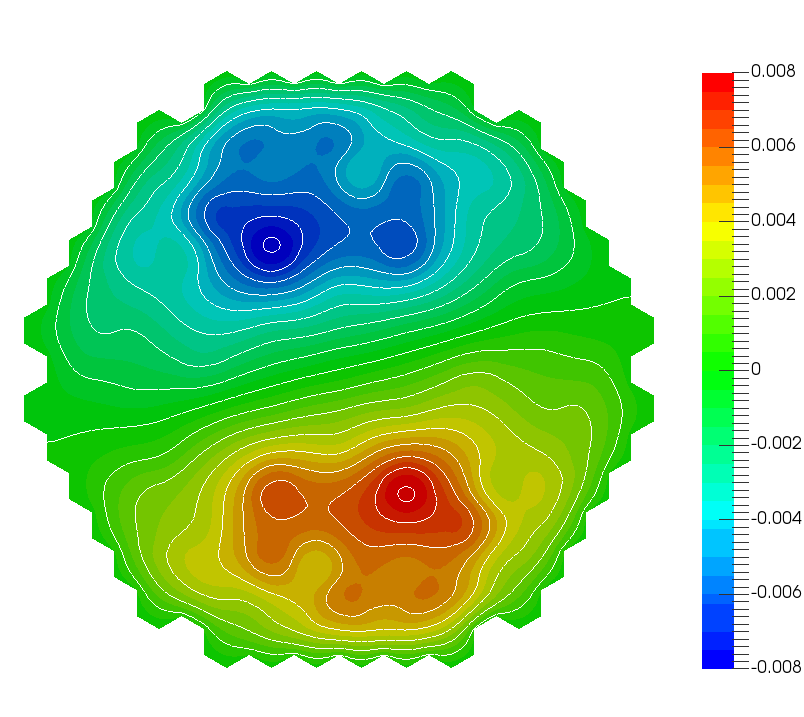
\includegraphics[width=1\linewidth]{5-1.png}} \\
%		\end{minipage}
%		\hfill
%		\begin{minipage}{0.49\linewidth}
%			\center{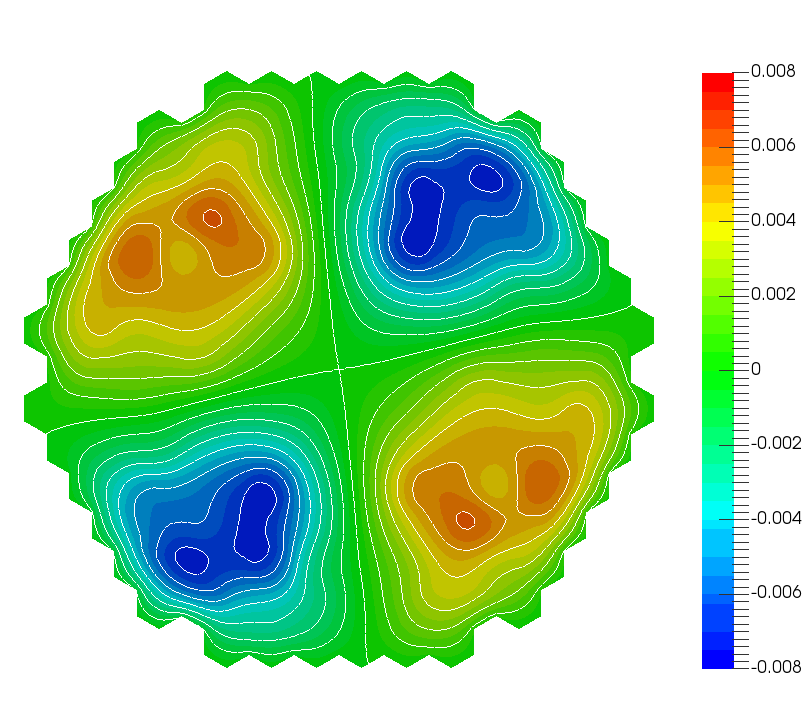
\includegraphics[width=1\linewidth]{5-2.png}} \\
%		\end{minipage}
%		\caption{Imaginary part of eigenfunctions $\varphi^{(2)}_1, \ - \varphi^{(3)}_1$ (left) and  real part of eigenfunctions $\varphi^{(4)}_1, \ \varphi^{(5)}_1$  (right).}
%		\label{fig:5}
%	\end{center}
%\end{figure}
%\end{frame}
%
%\begin{frame}
%\begin{figure}[!h]
%	\begin{center}
%		\begin{minipage}{0.49\linewidth}
%			\center{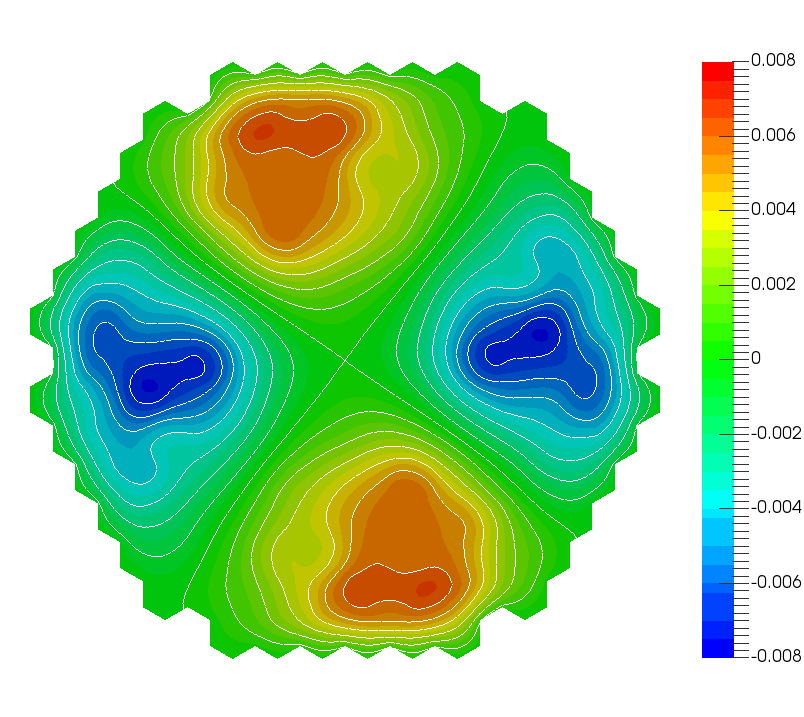
\includegraphics[width=1\linewidth]{6-1.png}} \\
%		\end{minipage}
%		\hfill
%		\begin{minipage}{0.49\linewidth}
%			\center{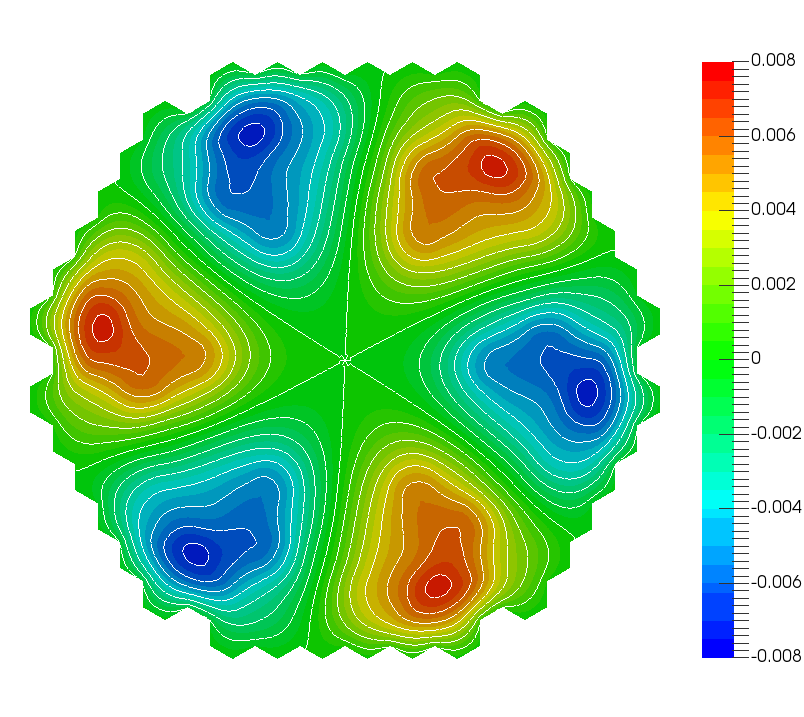
\includegraphics[width=1\linewidth]{6-2.png}} \\
%		\end{minipage}
%		\caption{Imaginary part of eigenfunctions $\varphi^{(4)}_1, \ - \varphi^{(5)}_1$ (left) and  eigenfunction $\varphi^{(6)}_1$  (right).}
%		\label{fig:6}
%  	\end{center}
%\end{figure}
%\end{frame}
%
%\begin{frame}
%\begin{figure}[!h]
%	\begin{center}
%		\begin{minipage}{0.49\linewidth}
%			\center{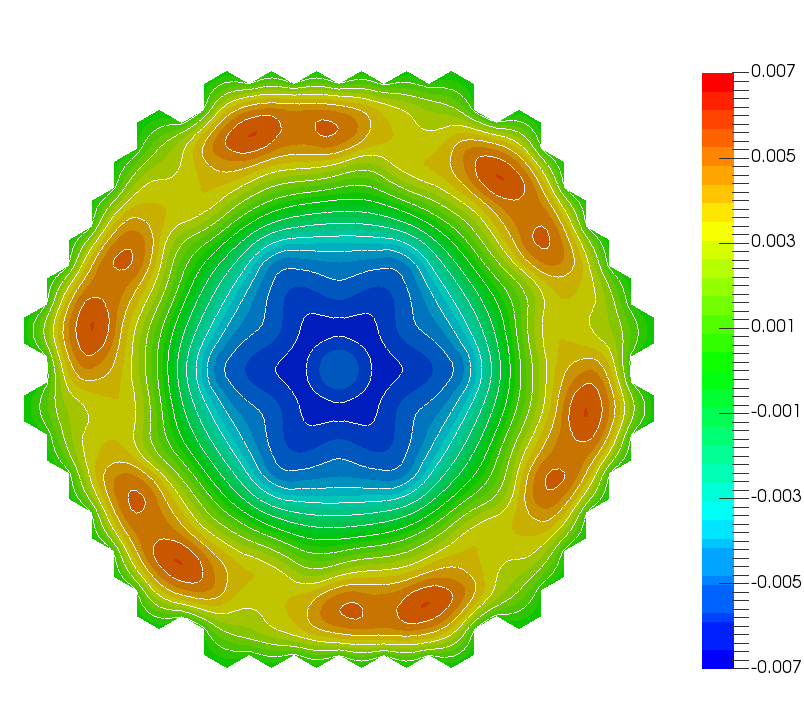
\includegraphics[width=1\linewidth]{7-1.png}} \\
%		\end{minipage}
%		\hfill
%		\begin{minipage}{0.49\linewidth}
%			\center{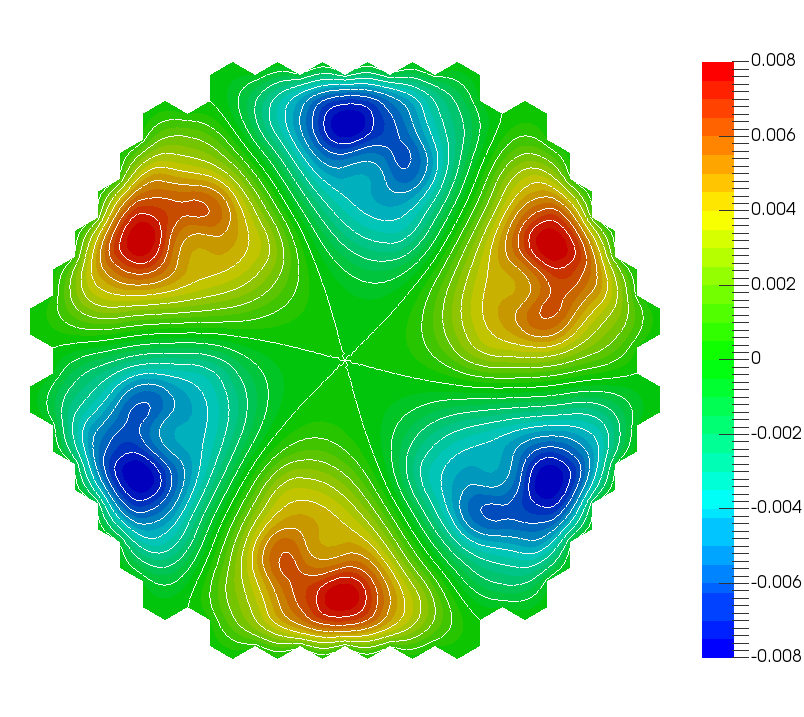
\includegraphics[width=1\linewidth]{7-2.png}} \\
%		\end{minipage}
%		\caption{The eigenfunction $\varphi^{(7)}_1$ (left) and  eigenfunction $\varphi^{(8)}_1$  (right).}
%		\label{fig:7}
%	\end{center}
%\end{figure}
%\end{frame}
%
%\begin{frame}
%\begin{figure}[!h]
%	\begin{center}
%		\begin{minipage}{0.49\linewidth}
%			\center{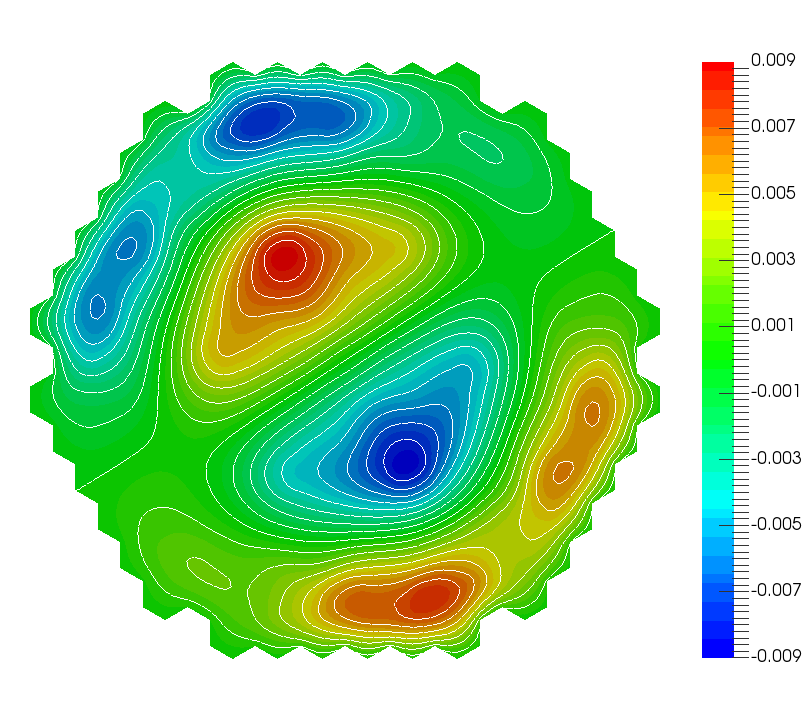
\includegraphics[width=1\linewidth]{8-1.png}} \\
%		\end{minipage}
%		\hfill
%		\begin{minipage}{0.49\linewidth}
%			\center{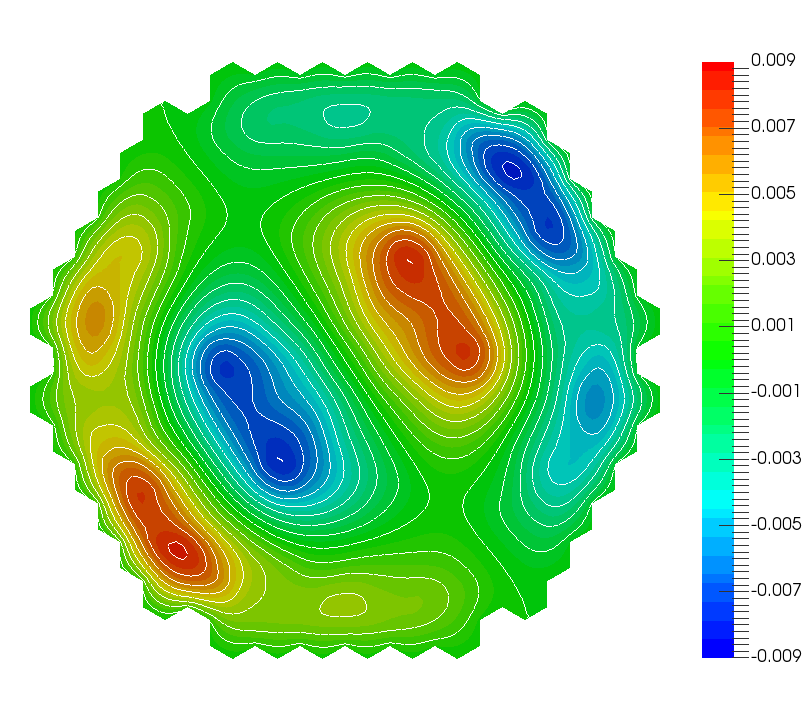
\includegraphics[width=1\linewidth]{8-2.png}} \\
%		\end{minipage}
%		\caption{Real part of eigenfunctions $\varphi^{(9)}_1, \ \varphi^{(10)}_1$ (left) and  imaginary part of eigenfunctions $\varphi^{(9)}_1, \ - \varphi^{(10)}_1$  (right).}
%		\label{fig:8}
%	\end{center}
%\end{figure}
%\end{frame}

\begin{frame}
	\begin{figure}[!h]
  		\begin{center}
			\begin{minipage}{0.49\linewidth}
				\center{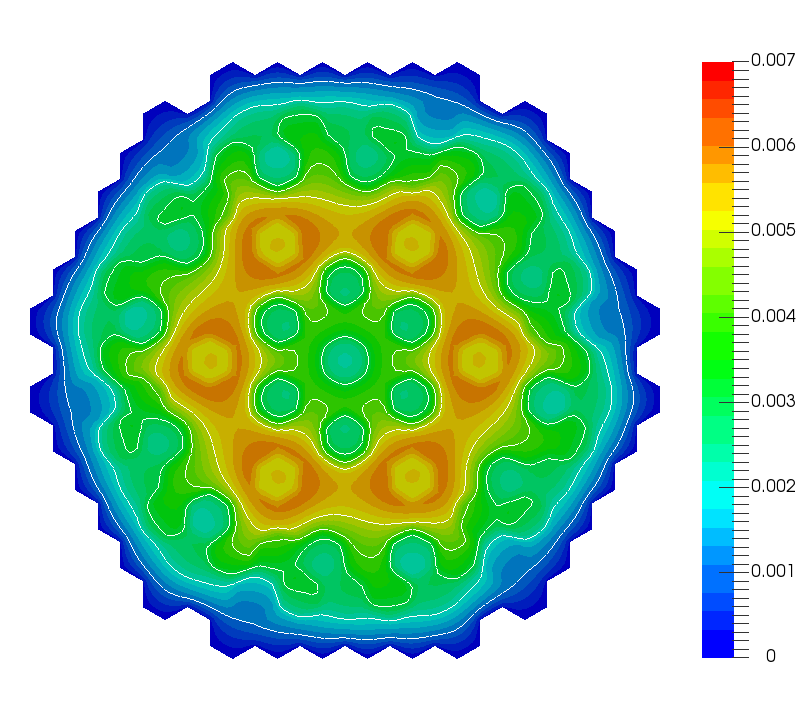
\includegraphics[width=1\linewidth]{9-1.png}} \\
			\end{minipage}
			\hfill
			\begin{minipage}{0.49\linewidth}
				\center{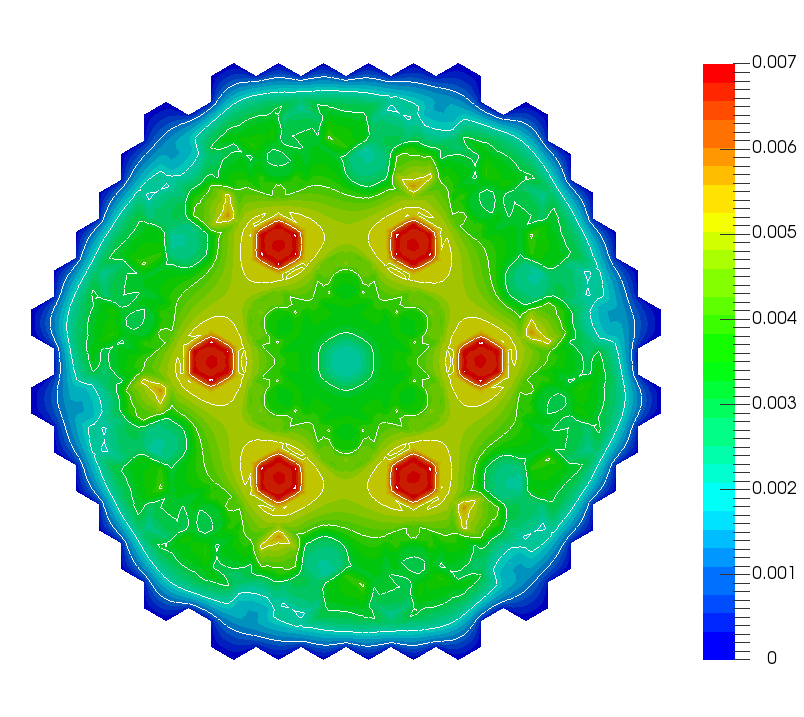
\includegraphics[width=1\linewidth]{9-2.png}} \\
			\end{minipage}
			\caption{The eigenfunction $\varphi^{(1)}_2$ (left) and the eigenfunctions $s^{(1)}$  (right).}
			\label{fig:9}
  		\end{center}
	\end{figure}
\end{frame}

%\begin{frame}{Adjoint spectral problem}
%\begin{table}[h]
%\caption{Eigenvalues $\alpha_n = \lambda_n^{(\alpha )}, \ n = 1,2, ..., 10$
%for direct and adjoint problems}
%\label{t-4}
%\begin{center}
%\begin{footnotesize}
%\begin{tabular}{rll}
%\hline
%$n$ & $\alpha_n$ for direct & $\alpha_n$ for adjoint \\
%\hline
%1 & -2.51280117966 & -2.51280117972 \\
%2,3 & 0.0355815000364 $\mp$ 5.80954455861e-06 & 0.0355815000365 $\mp$ 5.80954421646e-06 \\
%4,5 & 0.0644427013767 $\mp$ 1.41362187449e-06 & 0.0644427013767 $\mp$ 1.41362190730e-06 \\
%6 & 0.0702618501639 & 0.0702618501639 \\
%7 & 0.0714652882224 & 0.0714652882164 \\
%8 & 0.0726456060606 & 0.0726456060606 \\
%9,10 & 0.0734708921578 $\mp$ 4.02332269037e-08 & 0.0734708921578 $\mp$ 4.02332146248e-08 \\
%\hline
%\end{tabular}
%\end{footnotesize}
%\end{center}
%\end{table}
%\end{frame}
%
%\begin{frame}
%\begin{table}[h]
%\caption{Scalar product $(\phi_1^{(n)}, \phi_1^{(m)}), \ n, m = 1,2, ..., 5$}
%\label{t-5}
%\begin{center} 
%\begin{tabular}{c|rrrrr}
%\hline
%$n$\textbackslash$m$&1&2&3&4&5 \\
%\hline
%1 & 1.0e-00 & 1.3e-08 & 2.2e-08 & -3.8e-08 & 9.8e-09 \\ 
%2 & 1.3e-08 & 1.0e-00 & -1.6e-08 & -1.6e-08 & 1.4e-08  \\ 
%3 & 2.2e-08 & -1.6e-08 & 1.0e-00 & -9.8e-09 & -1.1e-08  \\ 
%4 & -3.8e-08 & -1.6e-08 & -9.8e-09 & 1.0e-00 & -3.9e-10  \\ 
%5 & 9.8e-09 & 1.4e-08 & -1.1e-08 & -3.9e-10 & 1.0e-00  \\ 
%6 & -1.8e-09 & 4.1e-08 & -1.8e-08 & -1.1e-08 & 2.9e-09  \\ 
%7 & 1.0e-02 & 1.2e-09 & 1.1e-08 & 1.4e-08 & -1.6e-08  \\ 
%8 & -3.2e-09 & -2.0e-07 & -3.3e-08 & 4.0e-09 & -1.9e-08  \\ 
%9 & -2.2e-08 & -3.1e-03 & -7.5e-03 & 3.0e-09 & 6.3e-09  \\ 
%10 & 1.6e-09 & 7.5e-03 & -3.1e-03 & -1.1e-08 & 6.3e-09  \\ 
%\hline
%\end{tabular}
%\end{center}
%\end{table}
%\end{frame}
%
%\begin{frame}
%\begin{table}[h]
%\caption{Scalar product $(\phi_1^{(n)}, \phi_1^{(m)}), \ n, m = 6,7, ..., 10$}
%\label{t-5}
%\begin{center} 
%\begin{tabular}{c|rrrrr}
%\hline
%$n$\textbackslash$m$&6&7&8&9&10 \\
%\hline
%1 & -1.8e-09 & 1.0e-02 & -3.2e-09 & -2.2e-08 & 1.6e-09 \\ 
%2 &  4.1e-08 & 1.2e-09 & -2.0e-07 & -3.1e-03 & 7.5e-03 \\ 
%3 &  -1.8e-08 & 1.1e-08 & -3.3e-08 & -7.5e-03 & -3.1e-03 \\ 
%4 &  -1.1e-08 & 1.4e-08 & 4.0e-09 & 3.0e-09 & -1.1e-08 \\ 
%5 &  2.9e-09 & -1.6e-08 & -1.9e-08 & 6.3e-09 & 6.3e-09 \\ 
%6 &  1.0e-00 & -4.2e-09 & -5.6e-03 & 4.1e-08 & -1.2e-07 \\ 
%7 &  -4.2e-09 & 1.0e-00 & -2.1e-09 & -1.8e-08 & 8.0e-09 \\ 
%8 &  -5.6e-03 & -2.1e-09 & 1.0e-00 & -5.2e-08 & 2.3e-07 \\ 
%9 &  4.1e-08 & -1.8e-08 & -5.2e-08 & 1.0e-00 & -5.5e-07 \\ 
%10 &  -1.2e-07 & 8.0e-09 & 2.3e-07 & -5.5e-07 & 1.0e-00 \\ 
%\hline
%\end{tabular}
%\end{center}
%\end{table}
%\end{frame}

%\begin{frame}
%Within the modal method, we can not rely on high accuracy when considering a relatively small number of dominant eigenvalues. Therefore, in the example under consideration, we can assume that the eigenvalues are real, and the corresponding eigenfunctions are orthogonal. 
%
%Instead of 
%\[
% b_n = \frac{1}{(\bm B_h \bm v_n, \widetilde{\bm v}_n)} (\bm u_h^s, \bm B_h \widetilde{\bm v}_n),
% \quad n = 1,2, ..., N_h 
%\]
%coefficients are used 
%\[
% b_n \approx  \frac{1}{(\bm c_n, \bm c_n)} (\bm c_h^s, \bm c_n),
% \quad n = 1,2, ..., N ,
%\]
%to approximate the initial condition.
%\end{frame}

%\subsection{Subcritical state}
%\begin{frame}{The symmetric perturbation}
%In the supercritical mode, due to the sufficiently large magnitude of the main eigenvalue, the regular regime of the reactor is rapidly developing, where 
%\[
% \bm u (\bm x, t) \approx a_1 \exp(-\alpha_1 t) \bm v_1^0 (\bm x) .
%\] 
%Here  $\bm v_1^0 (\bm x)$ is the first mode of the supercritical state. We consider the problem with the transition from this supercritical state at  $t_0 = 0$  to the subcritical state.
%
%The subcritical stage is characterized by a 15\% increase in the coefficient  
%$\Sigma_2$ for material 4 in the VVER-1000 test diffusion constants. 
%Thus, the dynamics of the reactor is as follows: 
%\[
% \Sigma_2 \longrightarrow 1.15 \Sigma_2 \quad (\mathrm{material} \ 4).
%\] 
%
%The initial state is characterized by specifying the initial conditions at $t_0 = 0$ as
%\[
% \bm u (\bm x, 0) = \bm v_1^0 (\bm x) . 
%\]
%\end{frame}
%
%\begin{frame}
%\begin{table}[h]
%\caption{Subcritical state: $\alpha_n = \lambda_n^{(\alpha )}, \ n = 1,2, ..., 5$}
%\label{t-6}
%\begin{center}
%\begin{tabular}{cccccc}
%\hline
%$p$ & $\kappa$ & $\alpha_1$ &  $\alpha_2, \alpha_3$ &  $\alpha_4, \alpha_5$ \\ 
%\hline
%   & 6 & 0.03602 & 0.05760 $\mp$ 1.49652e-06$i$ & 0.06890 $\mp$ 4.92606e-07$i$ \\ 
%1 & 24 & 0.02656 & 0.05502 $\mp$ 2.06007e-06$i$ & 0.06804 $\mp$ 1.01253e-06$i$ \\ 
%  & 96 & 0.02276 & 0.05411 $\mp$ 2.16813e-06$i$ & 0.06774 $\mp$ 1.03843e-06$i$ \\ 
%\hline
%   & 6 & 0.02250 & 0.05404 $\mp$ 1.81823e-06$i$ & 0.06772 $\mp$ 8.73562e-07$i$ \\ 
%2 & 24 & 0.02144 & 0.05380 $\mp$ 2.19400e-06$i$ & 0.06765 $\mp$ 1.04253e-06$i$ \\ 
%  & 96 & 0.02125 & 0.05376 $\mp$ 2.20812e-06$i$ & 0.06763 $\mp$ 1.04715e-06$i$ \\ 
%\hline
%   & 6 & 0.02139 & 0.05379 $\mp$ 2.22579e-06$i$ & 0.06764 $\mp$ 1.05369e-06$i$ \\ 
%3 & 24 & 0.02124 & 0.05376 $\mp$ 2.20883e-06$i$ & 0.06763 $\mp$ 1.04736e-06$i$ \\ 
%  & 96 & 0.02122 & 0.05376 $\mp$ 2.20951e-06$i$ & 0.06763 $\mp$ 1.04756e-06$i$ \\ 
%\hline
%\end{tabular}
%\end{center}
%\end{table}
%\end{frame}
%
%\begin{frame}
%\begin{table}[h]
%\caption{Subcritical state:  $\alpha_n = \lambda_n^{(\alpha )}, \ n = 6,7, ..., 10$}
%\label{t-7}
%\begin{center}
%\begin{tabular}{ccccccc}
%\hline
%$p$ & $\kappa$ & $\alpha_6$ &  $\alpha_7$ & $\alpha_8$ &  $\alpha_9, \alpha_{10}$ \\ 
%\hline
%   & 6 & 0.07276 & 0.07363 & 0.07369 & 0.07466 $\mp$ 2.47162e-08$i$ \\ 
%1 & 24 & 0.07222 & 0.07316 & 0.07329 & 0.07429 $\mp$ 1.08814e-08$i$ \\ 
%  & 96 & 0.07204 & 0.07301 & 0.07316 & 0.07417 $\mp$ 1.38093e-08$i$ \\
%\hline
%   & 6 & 0.07203 & 0.07300 & 0.07315 & 0.07416 $\mp$ 1.26708e-08$i$ \\ 
%2 & 24 & 0.07199 & 0.07296 & 0.07312 & 0.07413 $\mp$ 1.50527e-08$i$ \\ 
%  & 96 & 0.07198 & 0.07295 & 0.07312 & 0.07413 $\mp$ 1.49196e-08$i$ \\ 
%\hline
%   & 6 & 0.07198 & 0.07295 & 0.07312 & 0.07413 $\mp$ 1.52256e-08$i$ \\ 
%3 & 24 & 0.07198 & 0.07295 & 0.07312 & 0.07413 $\mp$ 1.49141e-08$i$ \\ 
%  & 96 & 0.07198 & 0.07295 & 0.07311 & 0.07413 $\mp$ 1.49178e-08$i$ \\ 
%\hline
%\end{tabular}
%\end{center}
%\end{table}
%\end{frame}
%
%\begin{frame}
%For an approximate solution, we use the following formulation:
%\[
% \bm u_N(\bm x, t) = 
% \sum_{n=1}^{N} b_n \exp(- \mathrm{Re} \, \alpha_n \, t) \bm v_n(\bm x) ,  
%\]
%where the coefficients $b_n, \ n = 1,2, ..., N$ are calculated according to the given initial condition.
%
%We distinguish two phases of the dynamic process: fast and slow. In the fast phase, the initial condition: from the function $\bm u(\bm x, 0)$ to the function $\bm u_N(\bm x, 0)$. 
%The slow phase is associated with the evolution of the solution according to above equation.
%Within the state change modal technology, the fast phase is not modeled at all.
%\end{frame}

\begin{frame}
\begin{figure}[!h]
  \begin{center}
    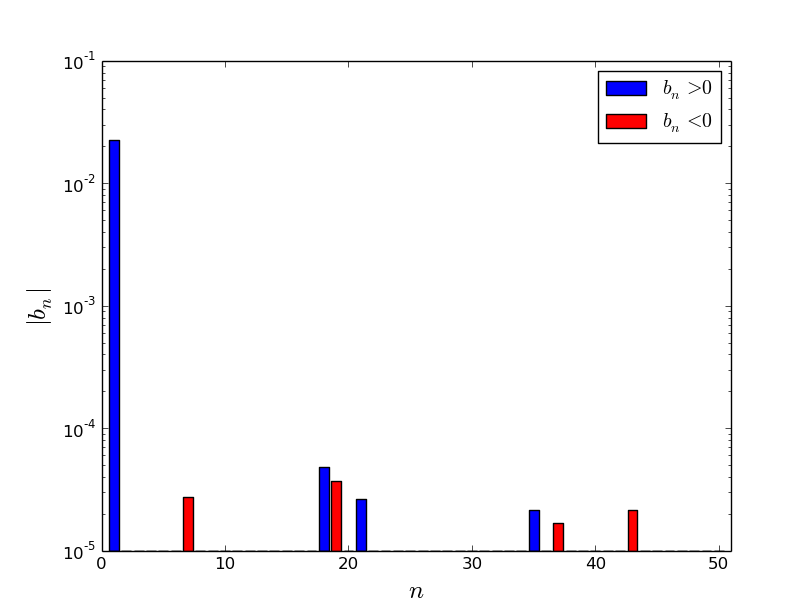
\includegraphics[width=0.85\linewidth] {10.png}
	\label{fig:10}
	\caption{Approximate solution coefficients}
  \end{center}
\end{figure} 
\end{frame}

\begin{frame}
\begin{figure}[!h]
  \begin{center}
\begin{minipage}{0.051\linewidth}
\center{1} \\
\end{minipage}
\hfill
\begin{minipage}{0.3\linewidth}
\center{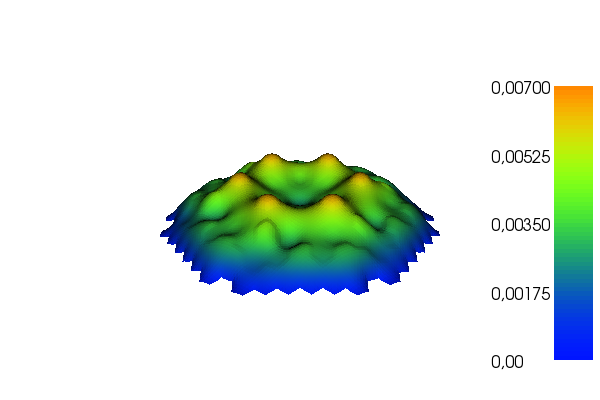
\includegraphics[width=1\linewidth]{11-11.png}} \\
\end{minipage}
\hfill
\begin{minipage}{0.3\linewidth}
\center{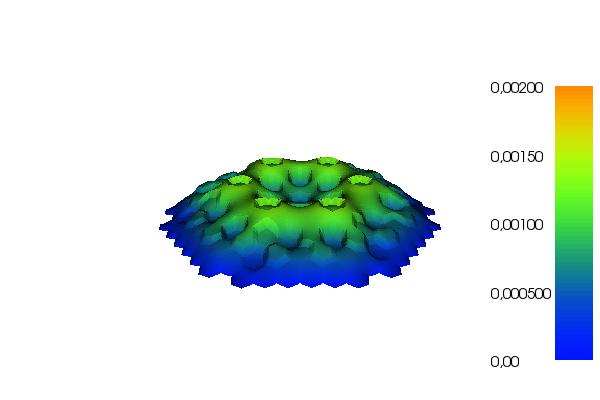
\includegraphics[width=1\linewidth]{11-12.png}} \\
\end{minipage}
\hfill
\begin{minipage}{0.3\linewidth}
\center{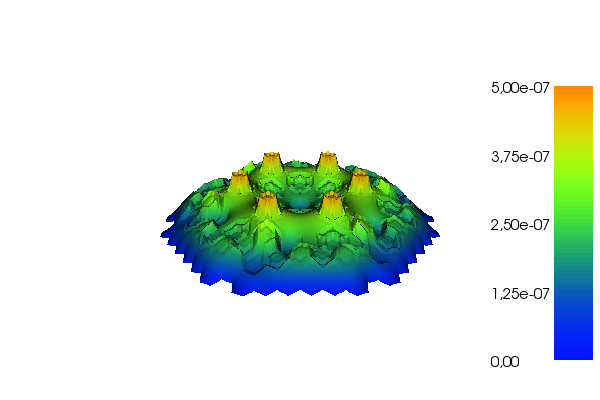
\includegraphics[width=1\linewidth]{11-13.png}} \\
\end{minipage}

\begin{minipage}{0.051\linewidth}
\center{2} \\
\end{minipage}
\hfill
\begin{minipage}{0.3\linewidth}
\center{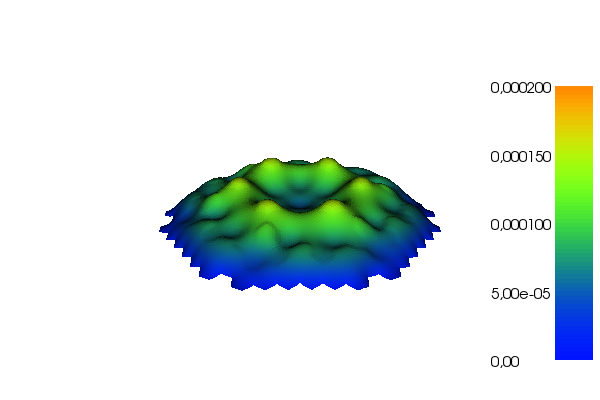
\includegraphics[width=1\linewidth]{11-21.png}} \\
\end{minipage}
\hfill
\begin{minipage}{0.3\linewidth}
\center{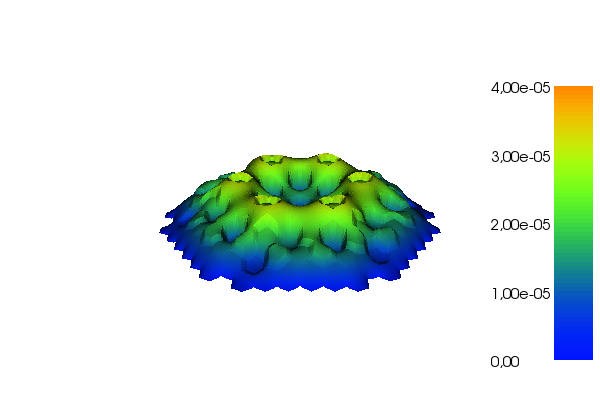
\includegraphics[width=1\linewidth]{11-22.png}} \\
\end{minipage}
\hfill
\begin{minipage}{0.3\linewidth}
\center{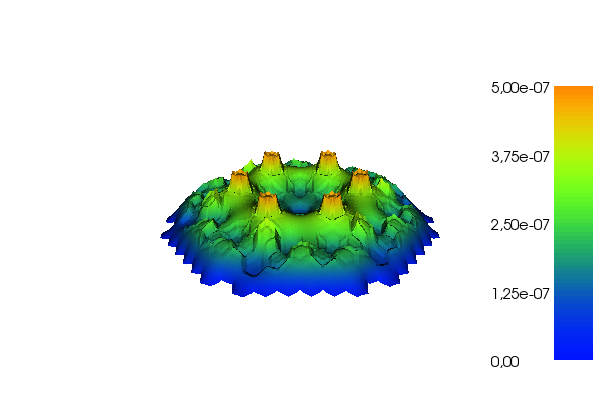
\includegraphics[width=1\linewidth]{11-23.png}} \\
\end{minipage}

\begin{minipage}{0.051\linewidth}
\center{~} \\
\end{minipage}
\hfill
\begin{minipage}{0.3\linewidth}
\center{a} \\
\end{minipage}
\hfill
\begin{minipage}{0.3\linewidth}
\center{b} \\
\end{minipage}
\hfill
\begin{minipage}{0.3\linewidth}
\center{c} \\
\end{minipage}
\hfill

\caption{Function $\bm u(\bm x, 0)$ (string 1) and function  $\bm u_N(\bm x, 0)$ (ctring 2):
a --- neutron flux of group 1, b --- neutron flux of group 2, c --- delayed neutrons source.}
\label{fig:11}
  \end{center}
\end{figure}
%Let us pay attention to the substantial restructuring of the solution, which is illustrated by large changes in the neutron flux amplitudes for the first and second groups.
\end{frame}

\begin{frame}{The asymmetric perturbation}
Consider a more complex transition to a subcritical state. The subcritical stage will be characterized by a different increase in the coefficient 
$\Sigma_2$ for material 4 in the diffusion constants in the upper and lower half of the reactor cross-section. Now let the reactor dynamics corresponds to the following transformation
\[
 \Sigma_2 \longrightarrow 
 \begin{cases}
 1.1 \Sigma_2, & \mathrm{material \ 4 \ (top \ part)}, \\
 1.2 \Sigma_2, & \mathrm{material \ 4 \ (bottom \ part)}.
 \end{cases}
\] 
All eigenvalues for this reactor state are real. 
\end{frame}

%\begin{frame}
%\begin{table}[h]
%\caption{Subcritical asymmetric state: $\alpha_n = \lambda_n^{(\alpha )}, \ n = 1,2, ..., 5$}
%\label{t-8}
%\begin{center}
%\begin{tabular}{ccccccc}
%\hline
%$p$ & $\kappa$ & $\alpha_1$ &  $\alpha_2$ & $\alpha_3$ &  $\alpha_4$ & $\alpha_5$ \\ 
%\hline
%   & 6 & 0.03347 & 0.05728 & 0.05788 & 0.06884 & 0.06889 \\ 
%1 & 24 & 0.02333 & 0.05467 & 0.05528 & 0.06797 & 0.06802 \\ 
%  & 96 & 0.01925 & 0.05374 & 0.05436 & 0.06768 & 0.06772 \\ 
%\hline
%   & 6 & 0.01894 & 0.05367 & 0.05429 & 0.06765 & 0.06770 \\ 
%2 & 24 & 0.01782 & 0.05343 & 0.05405 & 0.06758 & 0.06762 \\ 
%  & 96 & 0.01763 & 0.05339 & 0.05401 & 0.06757 & 0.06761 \\ 
%\hline
%   & 6 & 0.01777 & 0.05342 & 0.05404 & 0.06758 & 0.06762 \\ 
%3 & 24 & 0.01762 & 0.05339 & 0.05400 & 0.06757 & 0.06761 \\ 
%  & 96 & 0.01760 & 0.05338 & 0.05400 & 0.06757 & 0.06761 \\ 
%\hline
%\end{tabular}
%\end{center}
%\end{table}
%\end{frame}
%
%\begin{frame}
%\begin{table}[h]
%\caption{Subcritical asymmetric state:  $\alpha_n = \lambda_n^{(\alpha )}, \ n = 6,7, ..., 10$}
%\label{t-9}
%\begin{center}
%\begin{tabular}{cccccccc}
%\hline
%$p$ & $\kappa$ & $\alpha_6$ &  $\alpha_7$ & $\alpha_8$ &  $\alpha_9$ & $\alpha_{10}$ \\  
%\hline
%   & 6 & 0.07274 & 0.07355 & 0.07369 & 0.07464 & 0.07468 \\ 
%1 & 24 & 0.07220 & 0.07309 & 0.07329 & 0.07427 & 0.07430 \\
%  & 96 & 0.07202 & 0.07294 & 0.07316 & 0.07415 & 0.07419 \\ 
%\hline
%   & 6 & 0.07201 & 0.07293 & 0.07314 & 0.07414 & 0.07417 \\
%2 & 24 & 0.07197 & 0.07289 & 0.07311 & 0.07412 & 0.07415 \\ 
%  & 96 & 0.07196 & 0.07288 & 0.07311 & 0.07411 & 0.07414 \\ 
%\hline
%   & 6 & 0.07196 & 0.07289 & 0.07311 & 0.07411 & 0.07415 \\ 
%3 & 24 & 0.07196 & 0.07288 & 0.07311 & 0.07411 & 0.07414 \\ 
%  & 96 & 0.07196 & 0.07288 & 0.07311 & 0.07411 & 0.07414 \\ 
%\hline
%\end{tabular}
%\end{center}
%\end{table}
%\end{frame}

\begin{frame}
\begin{figure}[!h]
  \begin{center}
    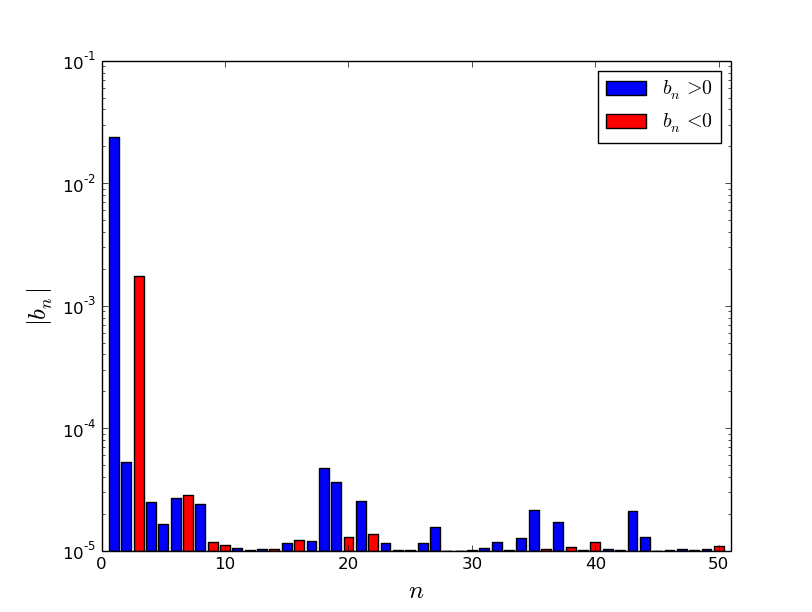
\includegraphics[width=0.85\linewidth] {12.png}
	\label{fig:12}
	\caption{Approximate solution coefficients}
  \end{center}
\end{figure} 
\end{frame}

\begin{frame}
\begin{figure}[!h]
  \begin{center}
\begin{minipage}{0.051\linewidth}
\center{1} \\
\end{minipage}
\hfill
\begin{minipage}{0.3\linewidth}
\center{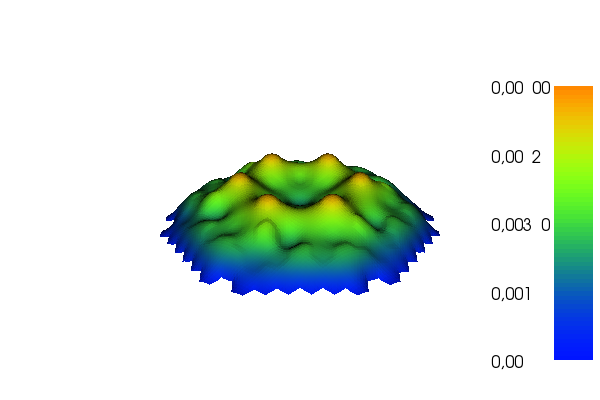
\includegraphics[width=1\linewidth]{13-11.png}} \\
\end{minipage}
\hfill
\begin{minipage}{0.3\linewidth}
\center{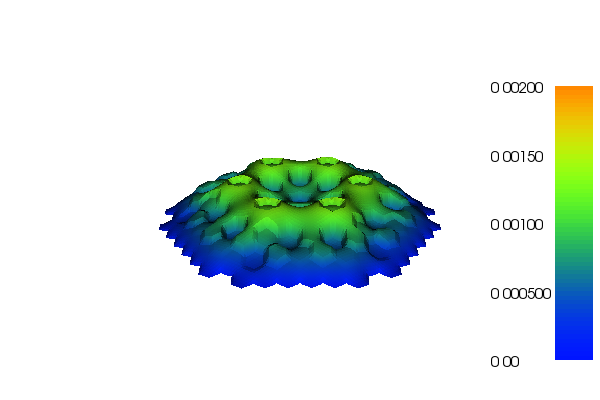
\includegraphics[width=1\linewidth]{13-12.png}} \\
\end{minipage}
\hfill
\begin{minipage}{0.3\linewidth}
\center{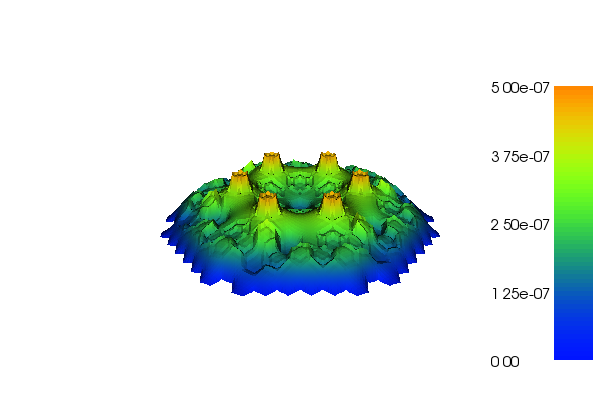
\includegraphics[width=1\linewidth]{13-13.png}} \\
\end{minipage}

\begin{minipage}{0.051\linewidth}
\center{2} \\
\end{minipage}
\hfill
\begin{minipage}{0.3\linewidth}
\center{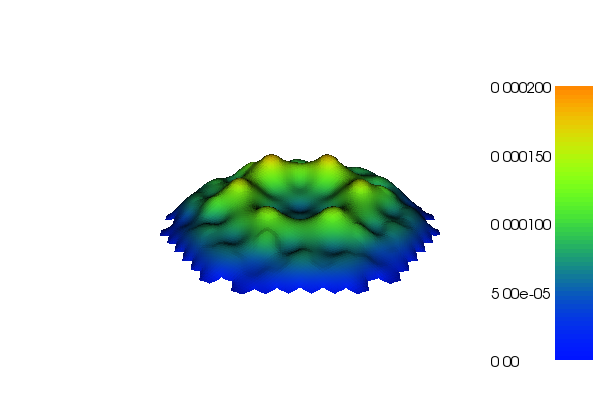
\includegraphics[width=1\linewidth]{13-21.png}} \\
\end{minipage}
\hfill
\begin{minipage}{0.3\linewidth}
\center{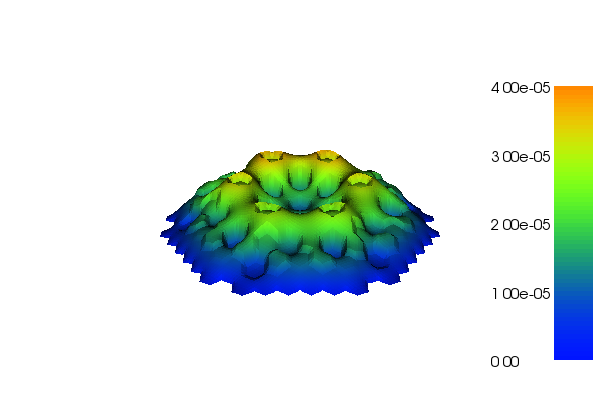
\includegraphics[width=1\linewidth]{13-22.png}} \\
\end{minipage}
\hfill
\begin{minipage}{0.3\linewidth}
\center{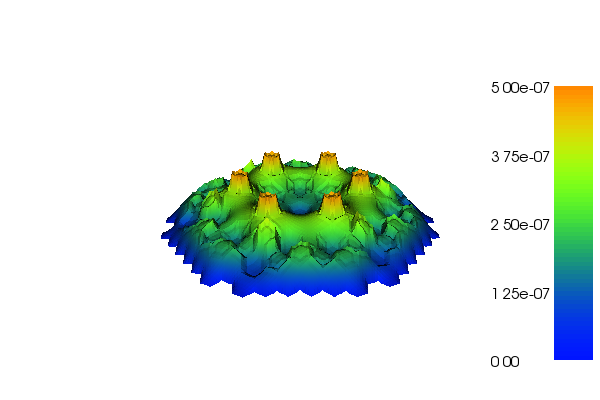
\includegraphics[width=1\linewidth]{13-23.png}} \\
\end{minipage}

\begin{minipage}{0.051\linewidth}
\center{~} \\
\end{minipage}
\hfill
\begin{minipage}{0.3\linewidth}
\center{a} \\
\end{minipage}
\hfill
\begin{minipage}{0.3\linewidth}
\center{b} \\
\end{minipage}
\hfill
\begin{minipage}{0.3\linewidth}
\center{c} \\
\end{minipage}
\hfill

\caption{Function $\bm u(\bm x, 0)$ (string 1) and function  $\bm u_N(\bm x, 0)$ (string 2) for asymmetric perturbation:
a --- neutron flux of group 1, b --- neutron flux of group 2, c --- delayed neutrons source.}
\label{fig:13}
  \end{center}
\end{figure}
%In the case under consideration, the approximate solution contains several modes and can not be described only by the first mode. 
%Calculations of the end of the fast phase are performed at  $N=10$. 
\end{frame}
\subsection{Comparison}
\begin{frame}{Fast stage of reactor state: neutronic power}
\begin{figure}[!h]
  \begin{center}
    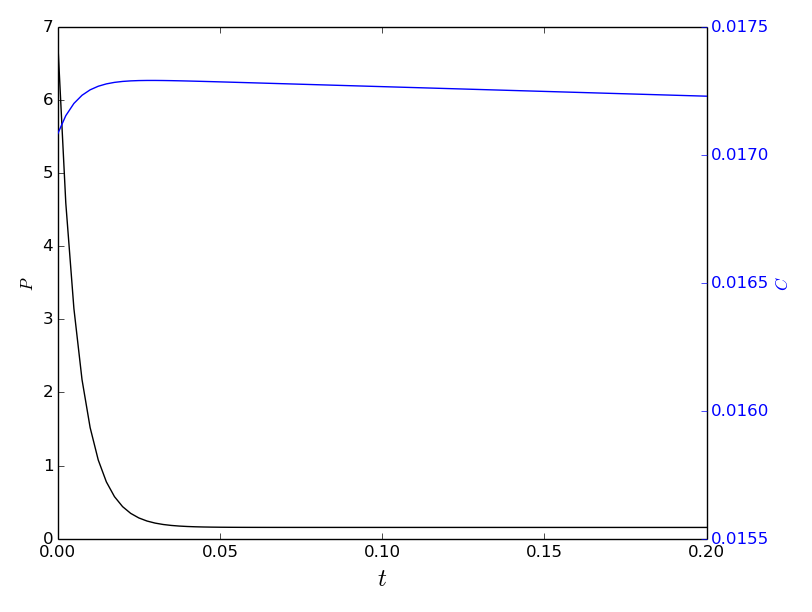
\includegraphics[width=0.9\linewidth] {14.png}
	\label{fig:14}
  \end{center}
\end{figure} 
\end{frame}

\begin{frame}{Slow stage of reactor state: neutronic power}
\begin{figure}[!h]
  \begin{center}
    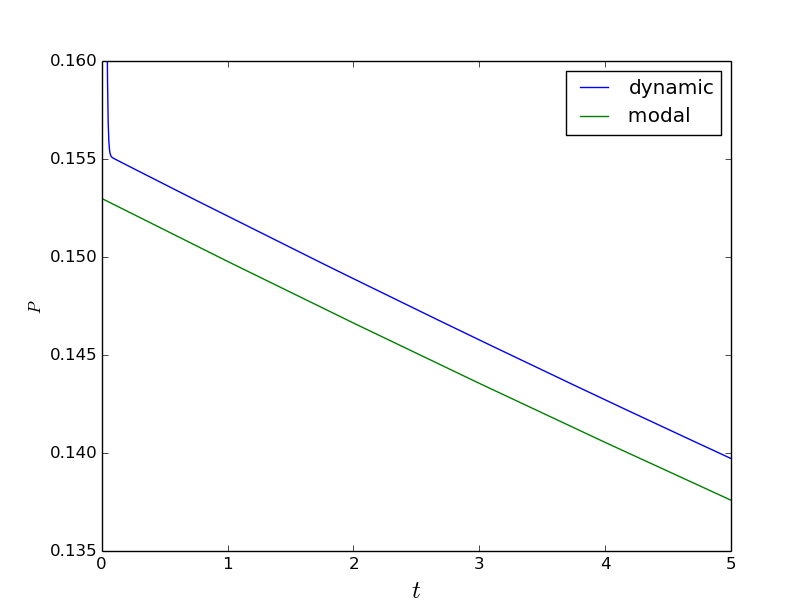
\includegraphics[width=0.85\linewidth] {15.png}
	\label{fig:15}
  \end{center}
\end{figure} 
\end{frame}

\begin{frame}{Slow stage of reactor state: delayed neutrons sourse}
\begin{figure}[!h]
  \begin{center}
    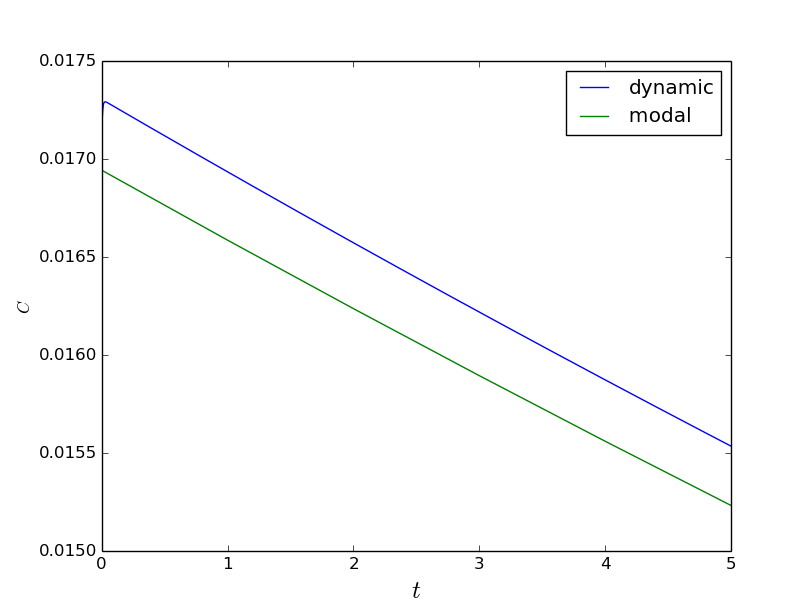
\includegraphics[width=0.85\linewidth] {16.png}
	\label{fig:16}
  \end{center}
\end{figure} 
\end{frame}

\begin{frame}{Slow stage of reactor state for the asymmetric perturbation: neutronic power}
\begin{figure}[!h]
  \begin{center}
    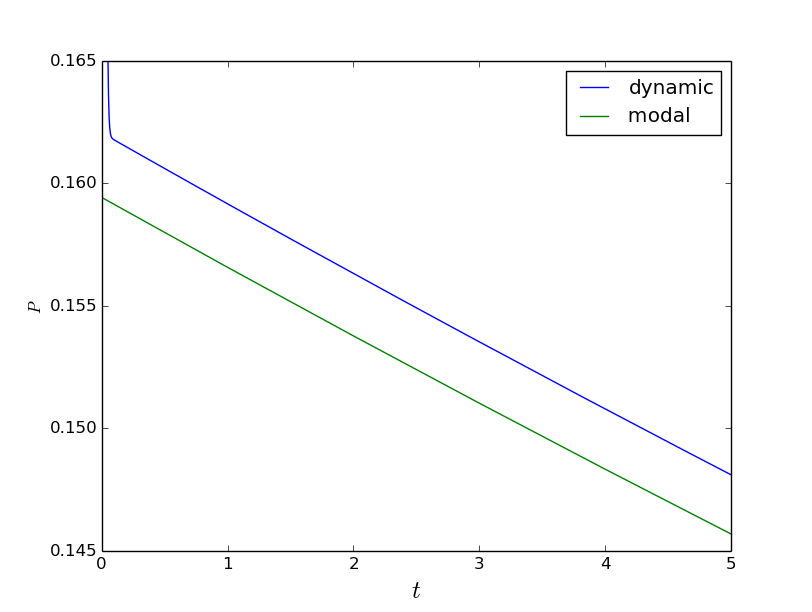
\includegraphics[width=0.85\linewidth] {17.png}
	\label{fig:17}
  \end{center}
\end{figure} 
\end{frame}

\begin{frame}{Slow stage of reactor state for the asymmetric perturbation: delayed neutrons sourse}
\begin{figure}[!h]
  \begin{center}
    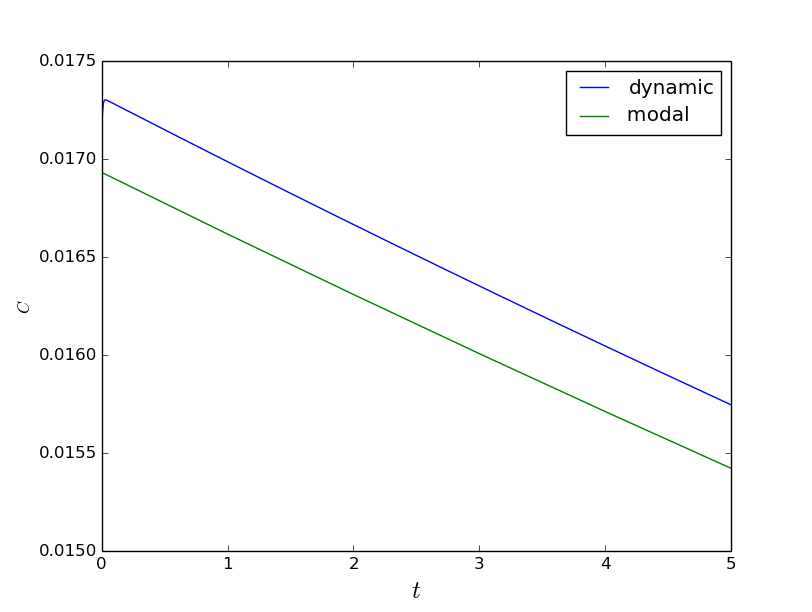
\includegraphics[width=0.85\linewidth] {18.png}
	\label{fig:18}
  \end{center}
\end{figure} 
\end{frame}

\section{Conclusion}
\begin{frame}{Conclusion}
\begin{itemize}
\item
The problem of simulation of reactor dynamic processes is considered on the basis of multigroup neutron diffusion equations accounting for delayed neutrons.
The modal approximation is used.
\item
In the developed SCM method a fast phase and slow phase is allocated
\item Offline calculation, online calculation
\item Finite Element Method, FEniCS, SLEPc
\item The modeling of the reactor state change as a transfer from one
state to another state, symmetric and assymetric perturbation
\item Comparison of the calculational results obtained by using two methods, one
based on modal approximation and another based on the full dynamics calculation
\end{itemize}

\begin{center}
Thank you for your attention!
\end{center}
\end{frame}

\end{document}
